% IMPORTANT: Please write various parts in different files, and then include
% them into this document.
% If you have a file called intro.tex then write: \include{intro}
% This is to avoid nasty merge conflicts, as well as to keep it tidy,
% modular, etc

\documentclass[11pt,a4paper,oneside]{report}

\usepackage{float} % have the position of pictures fixed

% Make bibliography appear in table of contents
\usepackage[nottoc,numbib]{tocbibind}

\usepackage{amsmath,amssymb,calc,ifthen,capt-of}


\usepackage[ampersand]{easylist}

\usepackage[table,usenames,dvipsnames]{xcolor} % for coloured cells in tables
\usepackage{color} % coloured text


% Allows us to click on links and references!
% http://tex.stackexchange.com/questions/73862/how-can-i-make-a-clickable-table-of-contents
\usepackage{hyperref}
\hypersetup{
    colorlinks,
    citecolor=black,
    filecolor=black,
    linkcolor=black,
    urlcolor=black
}

% Nice package for plotting graphs
% See excellent guide:
% http://www.tug.org/TUGboat/tb31-1/tb97wright-pgfplots.pdf
\usepackage{pgfplots}
\usetikzlibrary{plotmarks}
\usepackage{amsmath,graphicx}
\usepackage{epstopdf}
\usepackage{caption}
\usepackage{subcaption}

\pgfplotsset{compat = newest}

% highlight - useful for TODOs and similar
\usepackage{color}
\newcommand{\hilight}[1]{}%\colorbox{yellow}{#1}}


% margin size
\usepackage[margin=1in]{geometry}


\title{On a new metric to compare internal structures in biological networks}
\date{January 2014}
\author{
  Razvan Valentin Marinescu\\
  \texttt{rvm10@imperial.ac.uk}
}


\begin{document}
\belowdisplayskip=12pt plus 3pt minus 9pt
\belowdisplayshortskip=7pt plus 3pt minus 4pt
% General notes:

% Report Guidelines:
% http://www.doc.ic.ac.uk/lab/thirdyear/group-project/ReportGuidelines2012.pdf

% "This is more marketing than engineering. We don't want a diary"

% Tony: "How long? I don't know. Keep it short. 30 pages is absolutely fine.
% 40 a bit too much. 20 is a bit..."
% NOTE this excludes the appendices

% Keep it simple and to the point. Don't waffle

% Report is read by people who DONT know your work, though they are
% technically minded


\section*{Trade 1980 - 2010 - CCA results}


\definecolor{col1}{HTML}{5752FF} % blue
\definecolor{col2}{HTML}{05D1FF} % 
\definecolor{col3}{HTML}{85FFA3} % 
\definecolor{col4}{HTML}{C8FF85} % 
\definecolor{col5}{HTML}{F5FF85} % 
\definecolor{col6}{HTML}{FFA985} % 
\definecolor{col7}{HTML}{FF8585} % red


\begin{tabular}{ c | l }
canonical correlation &  0.945941034481261\\
p-values (asymptotic Wilks) & 0.0\\
\hline
"POP"& 0.73627568817745\\
"LE"& 0.716500474697832\\
"KIxRGDPLxPOP"& 0.660378185808367\\
"RGDPCHxPOP"& 0.653832159209968\\
"RGDPLxPOP"& 0.653755756195845\\
"RGDPL2xPOP"& 0.652259499516877\\
"KGxRGDPLxPOP"& 0.642377433267073\\
"KCxRGDPLxPOP"& 0.633027855098142\\
"KCxRGDPL"& 0.292515294847824\\
"XRAT"& 0.170830681533126\\
"RGDPCH"& 0.160785527502889\\
"RGDPL"& 0.160711435976867\\
"RGDPL2"& 0.16037796130068\\
"KGxRGDPL"& 0.158479027309231\\
"KIxRGDPL"& 0.104114574297674\\
"KC"& 0.0863445001675825\\
"KI"& -0.0161985756790376\\
"BCAperRGDPL"& -0.109531606033898\\
"KG"& -0.128677050226048\\
"BCA"& -0.149348165677686\\
"OPENK"& -0.265024465696308\\
\hline
\cellcolor{col2} "sig12" & 0.904560918713475\\
\cellcolor{col1}"sig10"&  0.893372614148734\\
\cellcolor{col2}"sig14"& 0.875359885181903\\
\cellcolor{col3}"sig17"& 0.859554707838637\\
\cellcolor{col1}"sig9"& 0.846921404801375\\
\cellcolor{col1}"sig11"& 0.837077663950148\\
\cellcolor{col3}"sig19"& 0.709659823734826\\
\cellcolor{col1}"sig4" &0.691975195223219\\
\cellcolor{col2}"sig16"& 0.674904586869997\\
\cellcolor{col1}"sig3" &0.630194434254492\\
\cellcolor{col3}"sig18"& 0.605640131807735\\
\cellcolor{col4}"sig24"& 0.597595307040999\\
\cellcolor{col2}"sig13"& 0.592465122198563\\
\cellcolor{col4}"sig22"& 0.545308255665041\\
\cellcolor{col4}"sig23"& 0.471536310817319\\
\cellcolor{col2}"sig15"& 0.438764964396065\\
\cellcolor{col3}"sig21"& 0.322210145884612\\
\cellcolor{col3}"sig20"& 0.289662264235416\\
\cellcolor{col5}"sig26"& 0.27067635709153\\
\cellcolor{col3}"sig6" &0.230567801167522\\
\cellcolor{col5}"sig27"& 0.153860022214748\\
\cellcolor{col4}"sig25"& 0.148231501271505\\
\cellcolor{col3}"sig5"& 0.112324390831594\\
\cellcolor{col6}"sig28"& -0.150155283916886\\
\cellcolor{col5}"sig1"& -0.163673627281325\\
\cellcolor{col6}"sig7"& -0.21277294295527\\
\cellcolor{col7}"sig2"& -0.486555451910386\\
\cellcolor{col7}"sig29"& -0.524621937849372\\
\cellcolor{col7}"sig8"& -0.637414244129602\\
\end{tabular}\\

\section*{Economic interpretation}

CCA shows that the good indicators such as RGDPL, POP, LE are positively correlated with the graphlets \{12,10,14,17,9,11,19,4,16, etc ..\}. On the other hand, the bad indicators correlate positively with graphlets {8,29,2,7,1,28}.
We now wonder what do graphlets from these two sets have in common. We first notice that graphlets {8,29,2,7,1,28} represent cliques {8,29,2} or almost cliques {7,1,28}. Since these graphlets are very densely connected, this suggests that the trading partners of small and poor countries are trading heavily with each other or form highly connected clusters. This suggests that \textbf{the majority of the trading partners of small and poor countries are the big and rich countries that are always trading heavily with each other}. 

This theory seems to be confirmed by taking a few small and poor countries and looking at their trading partners. Note that since the network has only 119 nodes, most of the poorest countries from Africa of South Asia have already been filtered out. Therefore, I have selected Morocco as a small and poor country relative to the others, although in reality it considered to have a medium level of development. Morocco's main trading partners are: {Saudi Arabia, China, France ,USA , Spain , Germany, Italy}. These countries are big and rich and every single pair of them clearly trade with each other. Similar results have been observed for other countries such as Bulgaria or Uruguay. Moreover, all of Morocco's trading partners are part of G20, a club of big and wealthy countries that collaborate with each other on economic matters. This leads us to a second theory: \textbf{since the trading partners of a small and poor country form highly connected clusters, these clusters represent big and rich economic groups such as G8, G20, OECD, Paris-club, BRIC}. Again, this is validated by selecting a few countries and looking at their neighbours. For example, the trading partners of Tunisia are Germany, France and Italy, all part of G8, G20, OECD and Paris-club. 

Regarding the first group of graphlets (that is \{12,10,14,17,9,11,19,4,16, etc ..\}), we wonder what they all have in common? We can find the answer quite easily by temporarily looking only at the 4-node graphlets, that is \{3,4,5,6,7,8\}. We find that the sparse graphlets \{3,4\} have a high positive weight, medium-dense graphlets \{5,6\} have a low positive weight (0.11 and 0.23), while dense graphlets \{7,8\} have a negative weight. This suggests that the graphlets are ordered according to how dense they are, from sparsely connected graphlets (coloured in blue) having a high positive weight to densely connected graphlets (coloured in red) having a negative weight. 

Now that we now know to interpret the positively weighted part of the graphlet vector as sparse graphlets, canonical correlation tells us that the trading partners of big and wealthy countries have a lot of sparse graphlets in their neighbourhood. The economic reason for this is because \textbf{big and rich countries like USA, China, Russia are trading with a lot of small, isolated countries which in turn do not trade with each other}. This theory is supported by a closer analysis with Cytoscape. Using this software I have found that the clustering coefficient of a country is inversely correlated with the wealth and size of that country, suggesting that big and rich countries have a relatively much sparser neighbourhood.


The population of the country seems to be quite an important factor for determining whether it will have a neighbourhood rich in sparse graphs because of the following two reasons:
\begin{itemize}
 \item In the indicators vector, population has the weight with the highest magnitude: 0.73
 \item Most of the other indicators that have a high positive weight are obtained by mutiplying population with other indicators (KIxRGDPLxPOP, RGDPCHxPOP). It should be noted that this is also the case in Omer et al's paper "Revealing the hidden language" ...
\end{itemize}


\begin{figure}[H]
  \centering
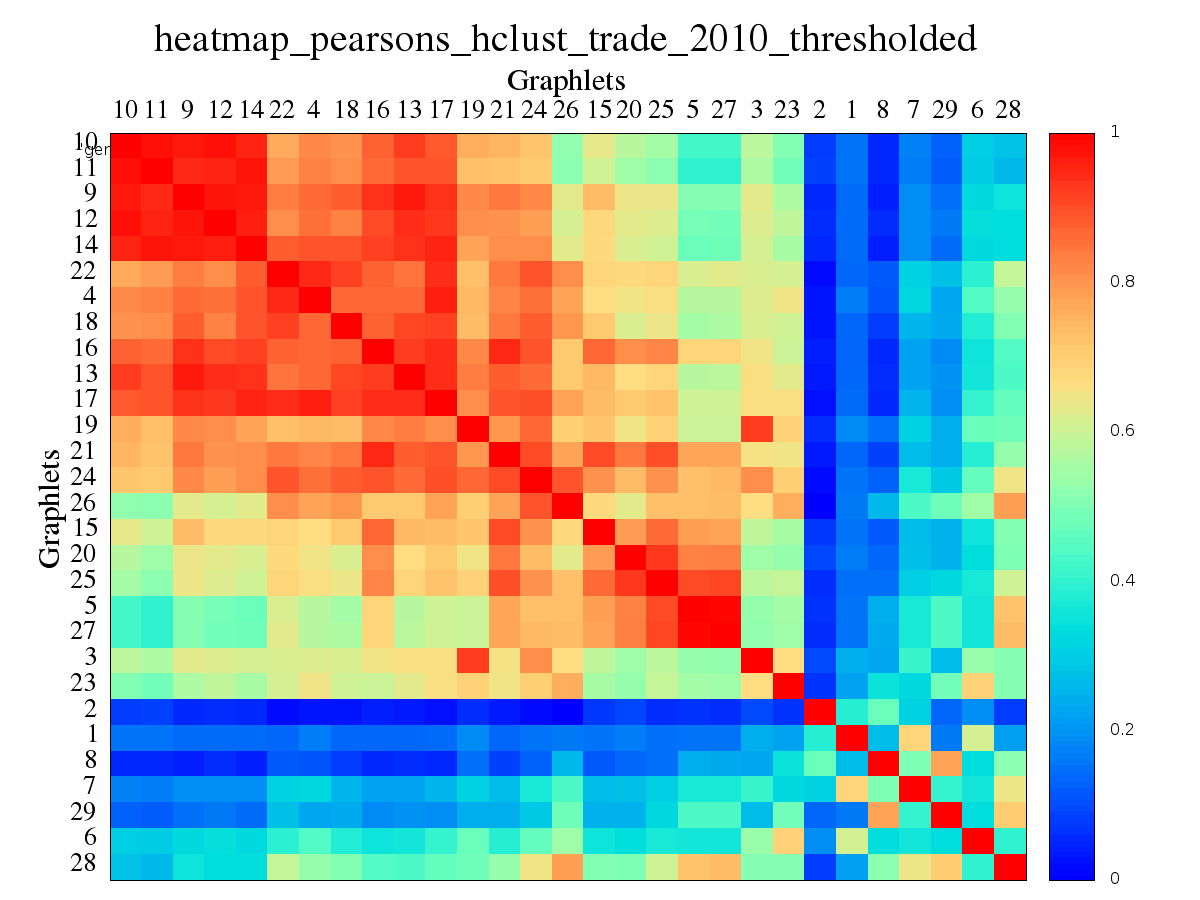
\includegraphics[scale=0.4]
{../code/final_results_norm1/trade_2010_thresholded/heatmap_pearsons_hclust_trade_2010_thresholded.png}
\caption{}
\label{fig:trade}
\end{figure}

In the trade network, we can observe several clusters of graphlets that ahave been formed along the diagonal:
\begin{itemize}
 \item \textbf{A}: Cluster made of graphlets \{10,11,9,12,14\}. These are all sparse graphlets, and CCA analysis shows that these graphlets are correlated with big and rich countries. Note that graphlet 9 does not always correlate in previous years. All apart from G9 contain a C4.
 \item \textbf{B}: A slightly similar cluster that is also correlated with the one above is \{22,4,18,16,13,17\}. These graphlets all contain a C4 as a subgraph, so perhaps that is the reason for being correlated together.
 \item \textbf{C}: Another cluster is formed by graphlets \{5,25,27,20\}, with graphlet 20 being added because it is highly correlated especially in other years. These graphlets all contain a cycle of length 4 (S4).  
\end{itemize}

\section*{Economic interpretation}

The graphlets from cluster \textbf{A} are all sparse graphs that are associated with big and wealthy countries, according to the CCA analysis (see below). The graphlets that are associated with small and poor countries are the dense graphlets \{ 2,8,29,1,7,28 \}. These dense graphlets are however not correlated with each other. This tells us that the positive topological attributes (sparse graphlets) correlate positively with each other, while negative attributes (dense graphlets) dont't correlate with each other and correlate negatively with the positive ones (this can't be noticed from the plot because the correlation matrix is normalized, but in the original version the dense graphlets correlate negatively with the sparse ones). This in turn means, that if a country has a positive attribute, it will be prone to have more of those positive topological attributes (highly positive correlation), which will in turn lead to make it richer. Similarly, a negative topological attribute will be negatively correlated with a positive attribute, which means that if a country has a negative attribute it will be less like to have a positive attribute at the same time. Therefore, if a country is poor this will somehow stop or delay it from becoming richer. This suggests that the \textbf{Rich countries get richer, while poor countries get poorer}. The phrase is generally attributed to a free market system (capitalism) (Wikipedia, Karl Marx - law of increasing poverty). 

Most of the graphlets from group A also correlate with one another in other network classes such as Knuth's literature networks. For example, in Anna Karenina graphlets 10,11,12 and 9 also also correlated and form a cluster. Similarly, graphlet from group C are also correlated in literature networks (\{5,25,27\} in Anna Karenina and \{5,27\} in David Copperfield). Therefore there are two conclusions I can draw from here:
\begin{itemize}
 \item The trade networks and the literature networks might have some common property. What I have noticed so far is that these networks have a small number of nodes. This would in turn cause the number of samples for calculating the Pearson's correlation matrix to also be small. Therefore, the reason for the clear clusters might also be because there are less outliers, since only the strong connections are kept. To test this out I compared 2 versions of Anna Karenina. One with a small number of nodes and another with 5x more nodes. The one with a small number of nodes indeed has much clearer clusters compared to the one with a bigger number of nodes.  
 \item The graphlets get clustered because they have a common sub-structure in common (ex: Cluster B contains C4). 
\end{itemize}

Because of the above two points, I do not believe there can be attributed any roles to countries in this scenario. Another aspect is that our GCV metric is much more abstract than the equivalent GDV signature with orbits, since it gives us information about the trading partners of a particular country, but not about the country itself.


\section*{Trade network over the years}

\subsection*{1962 to 1972}

\begin{figure}[H]
  \centering
  \label{fig:asafa}
  
  \subfloat{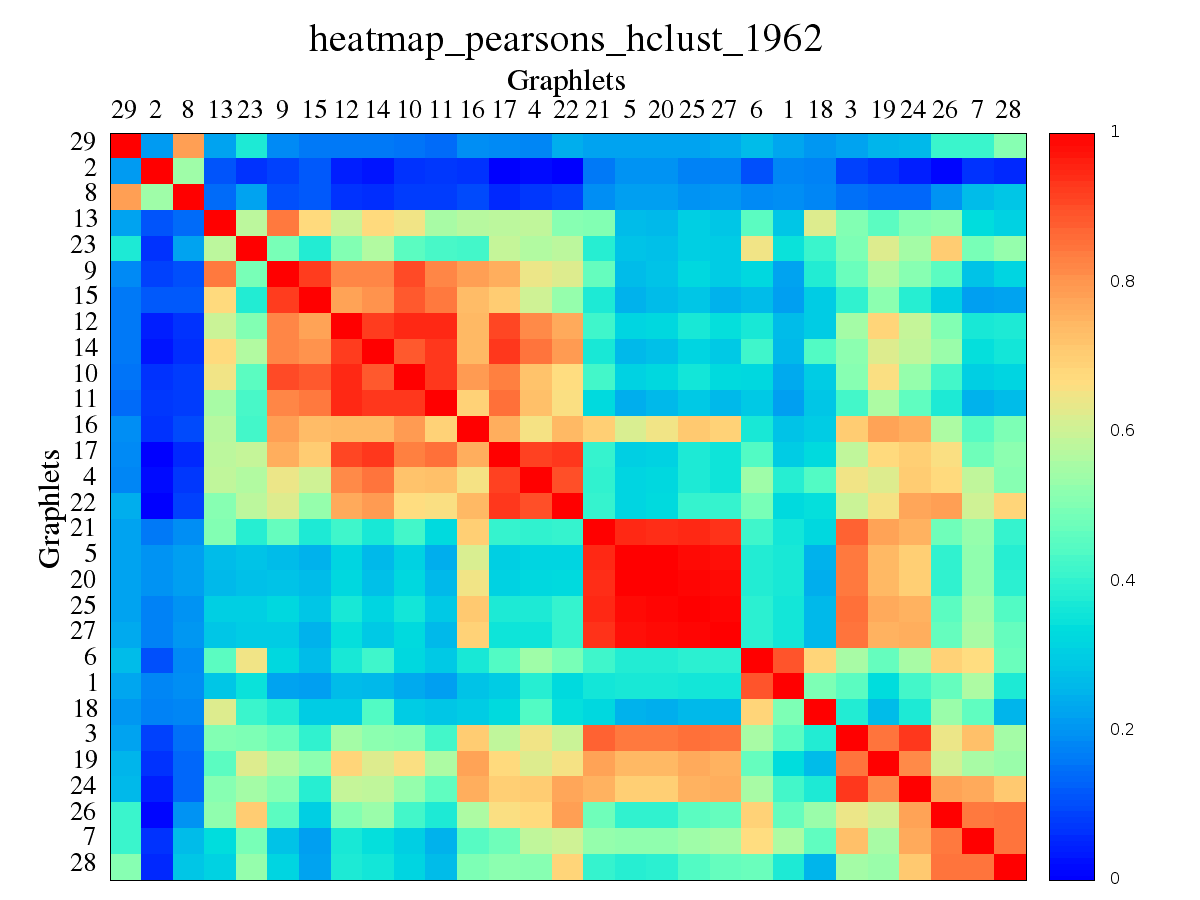
\includegraphics[width=70mm]{../code/final_results_norm1/all_trade_thresh/heatmap_pearsons_hclust_1962.png}}
  \subfloat{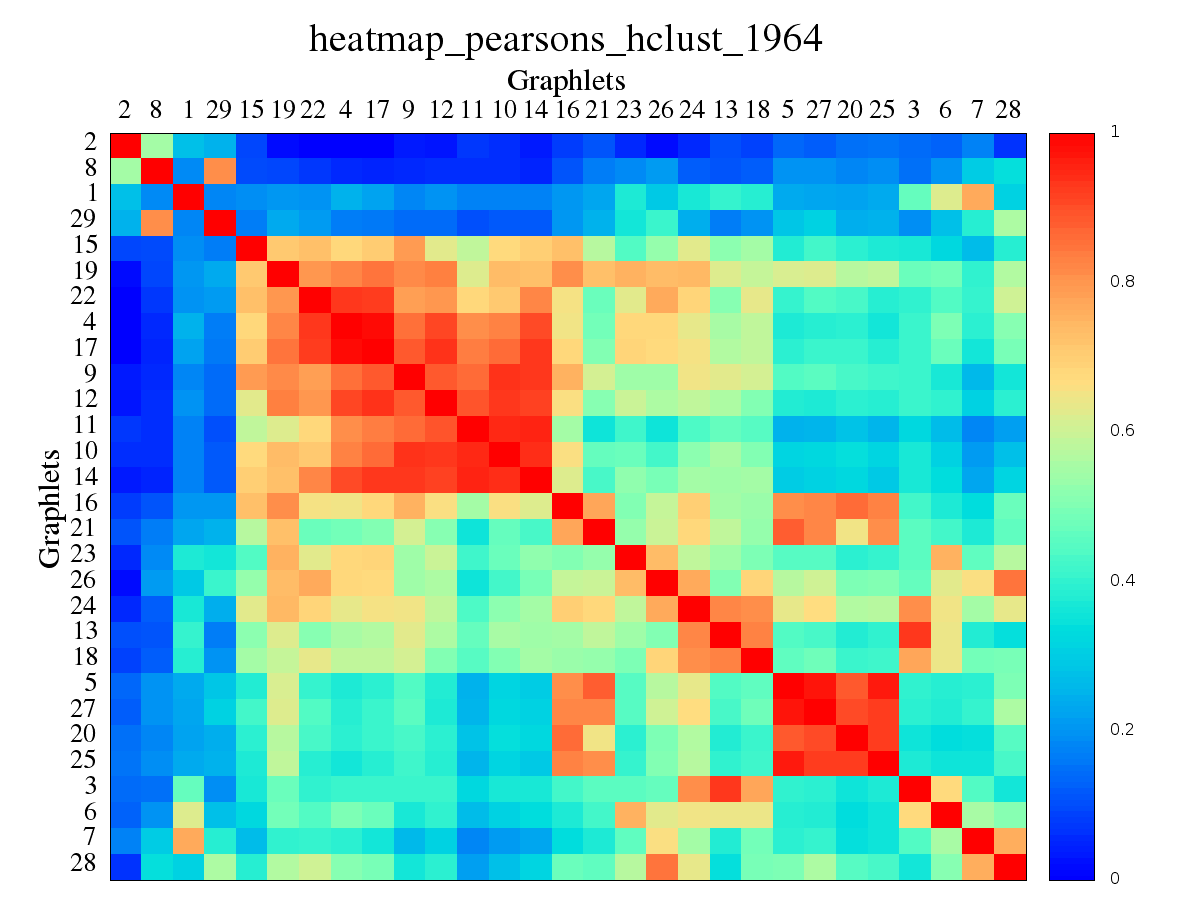
\includegraphics[width=70mm]{../code/final_results_norm1/all_trade_thresh/heatmap_pearsons_hclust_1964.png}}
  \\
  \subfloat{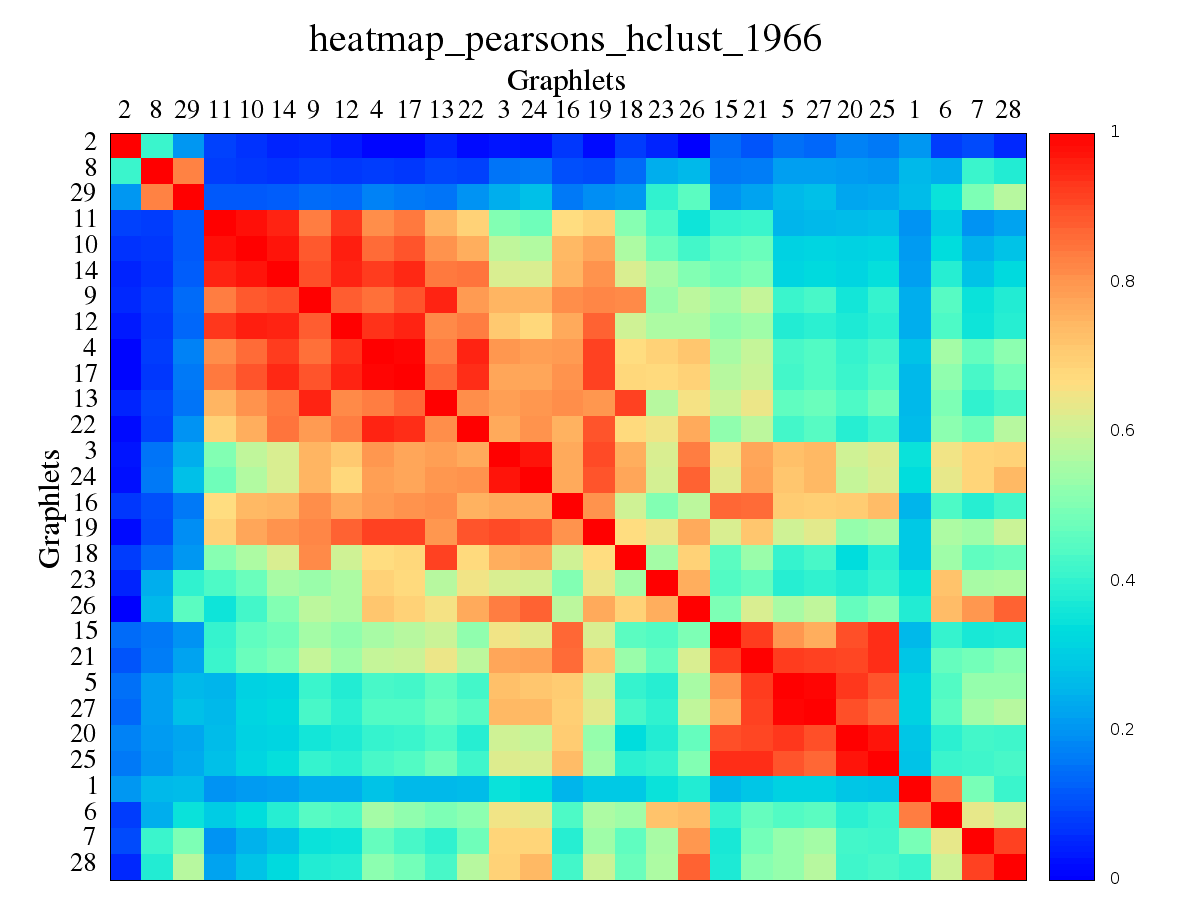
\includegraphics[width=70mm]{../code/final_results_norm1/all_trade_thresh/heatmap_pearsons_hclust_1966.png}}
  \subfloat{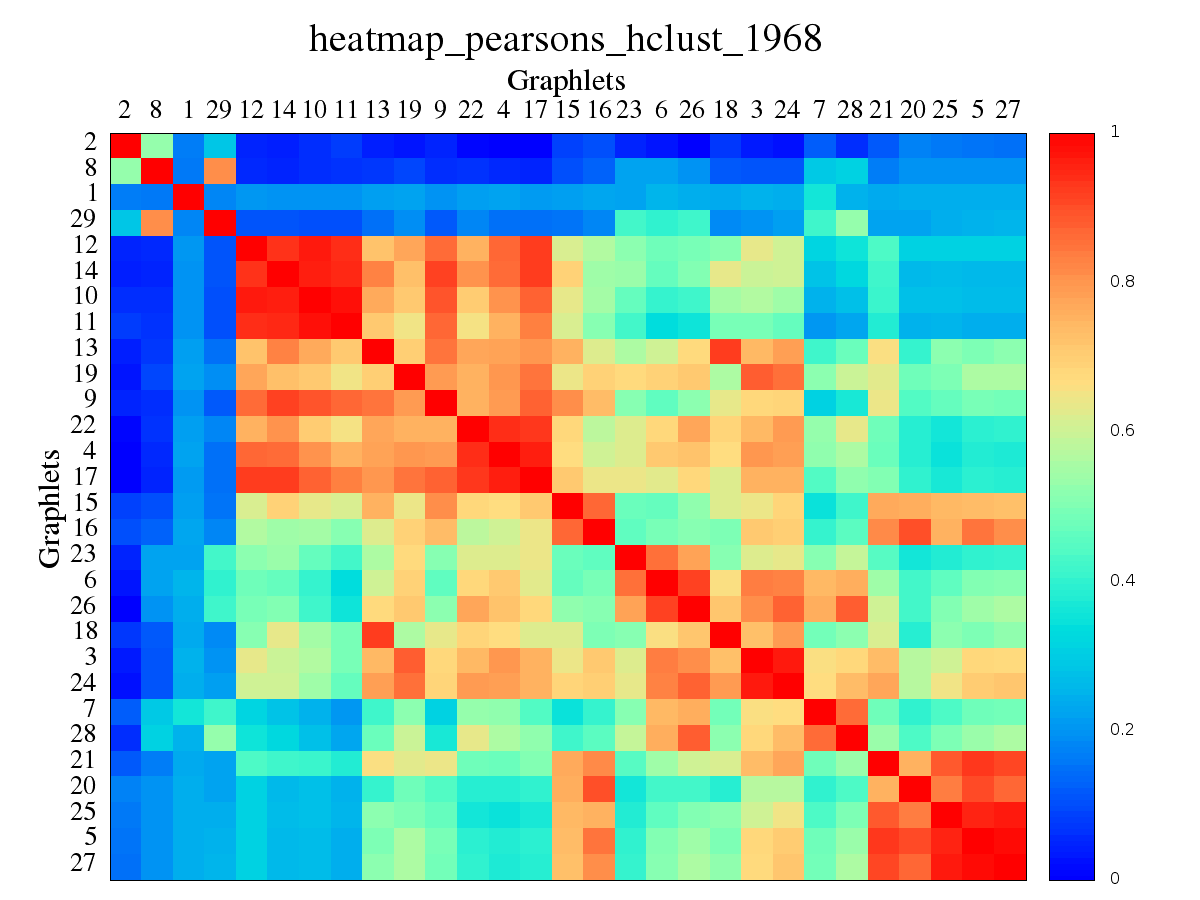
\includegraphics[width=70mm]{../code/final_results_norm1/all_trade_thresh/heatmap_pearsons_hclust_1968.png}}
  \\
  \subfloat{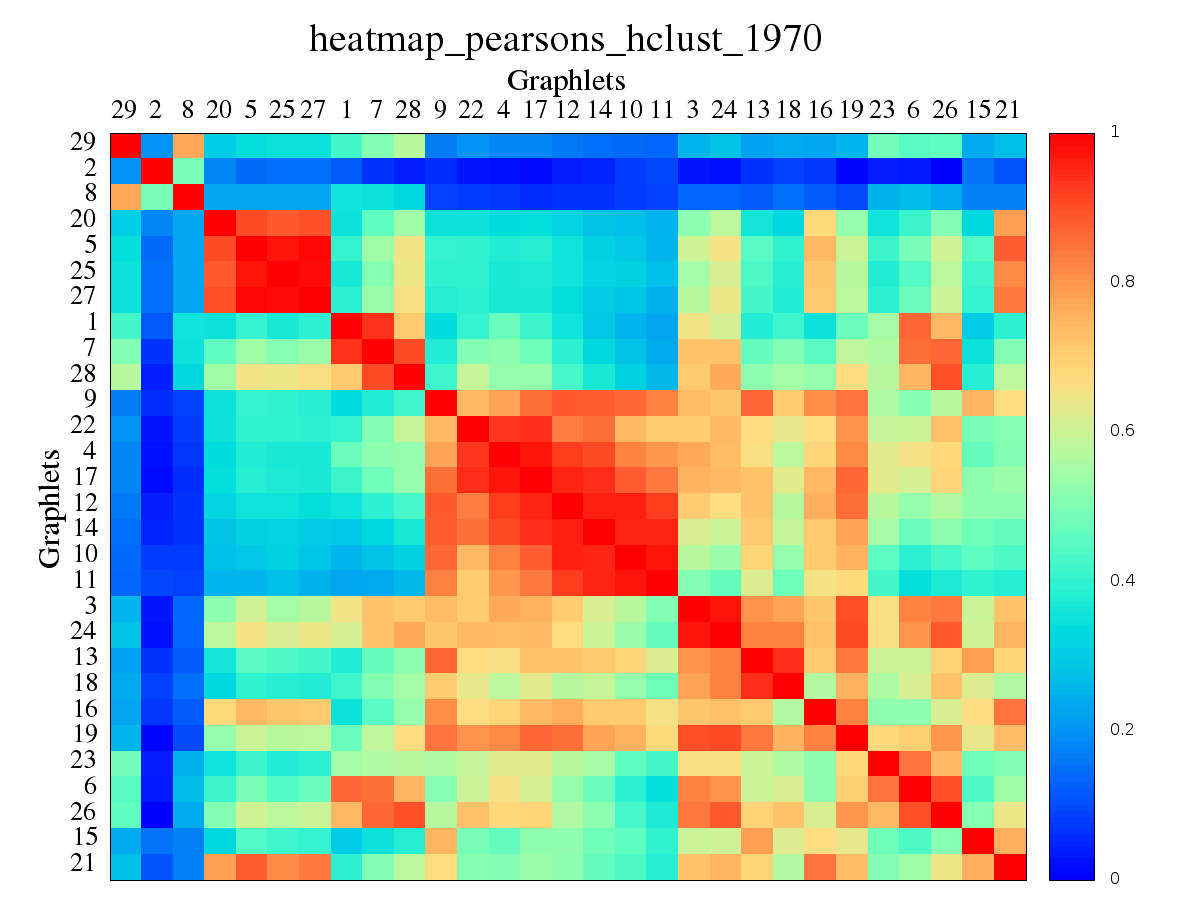
\includegraphics[width=70mm]{../code/final_results_norm1/all_trade_thresh/heatmap_pearsons_hclust_1970.png}}
  \subfloat{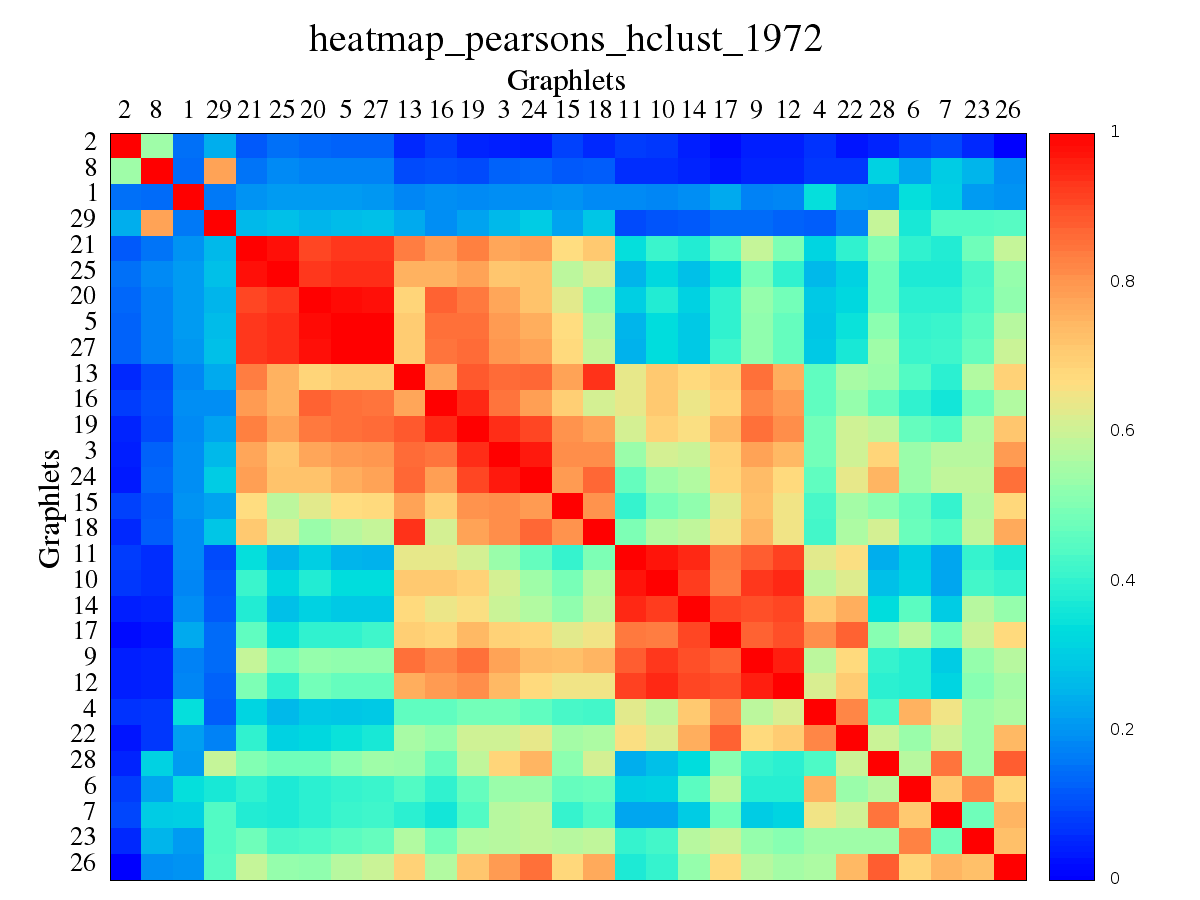
\includegraphics[width=70mm]{../code/final_results_norm1/all_trade_thresh/heatmap_pearsons_hclust_1972.png}}

\end{figure}


\subsection*{1974 to 1984}

\begin{figure}[H]
  \centering
  \label{fig:asafa}
  
  \subfloat{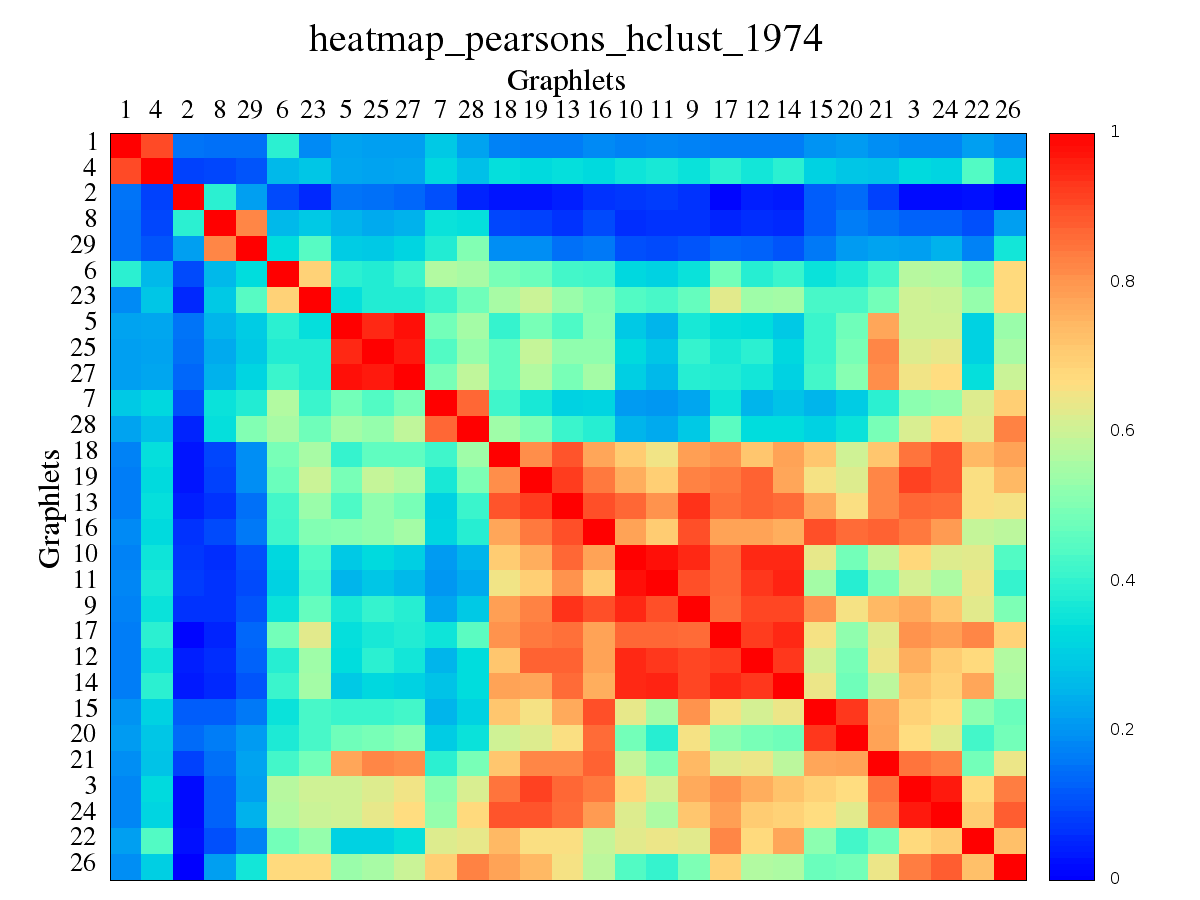
\includegraphics[width=70mm]{../code/final_results_norm1/all_trade_thresh/heatmap_pearsons_hclust_1974.png}}
  \subfloat{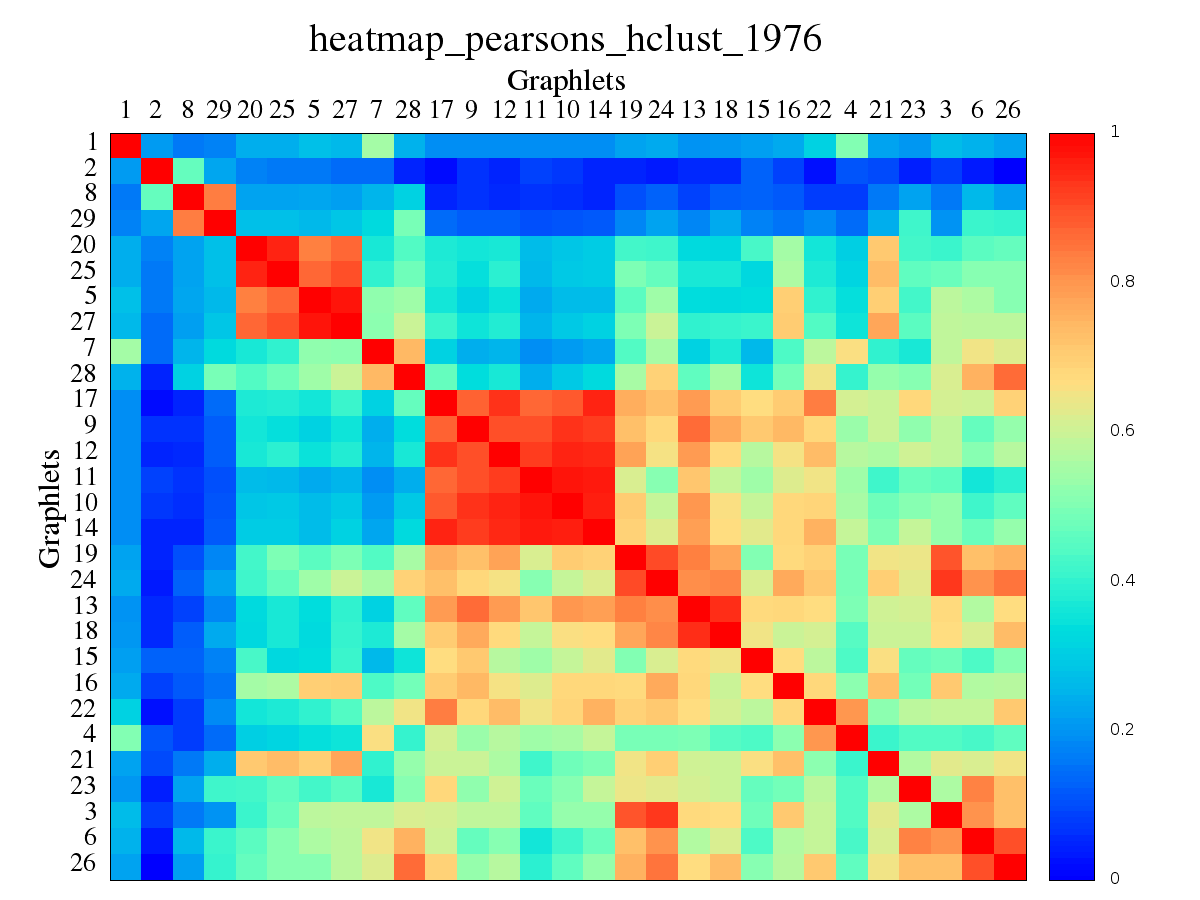
\includegraphics[width=70mm]{../code/final_results_norm1/all_trade_thresh/heatmap_pearsons_hclust_1976.png}}
  \\
  \subfloat{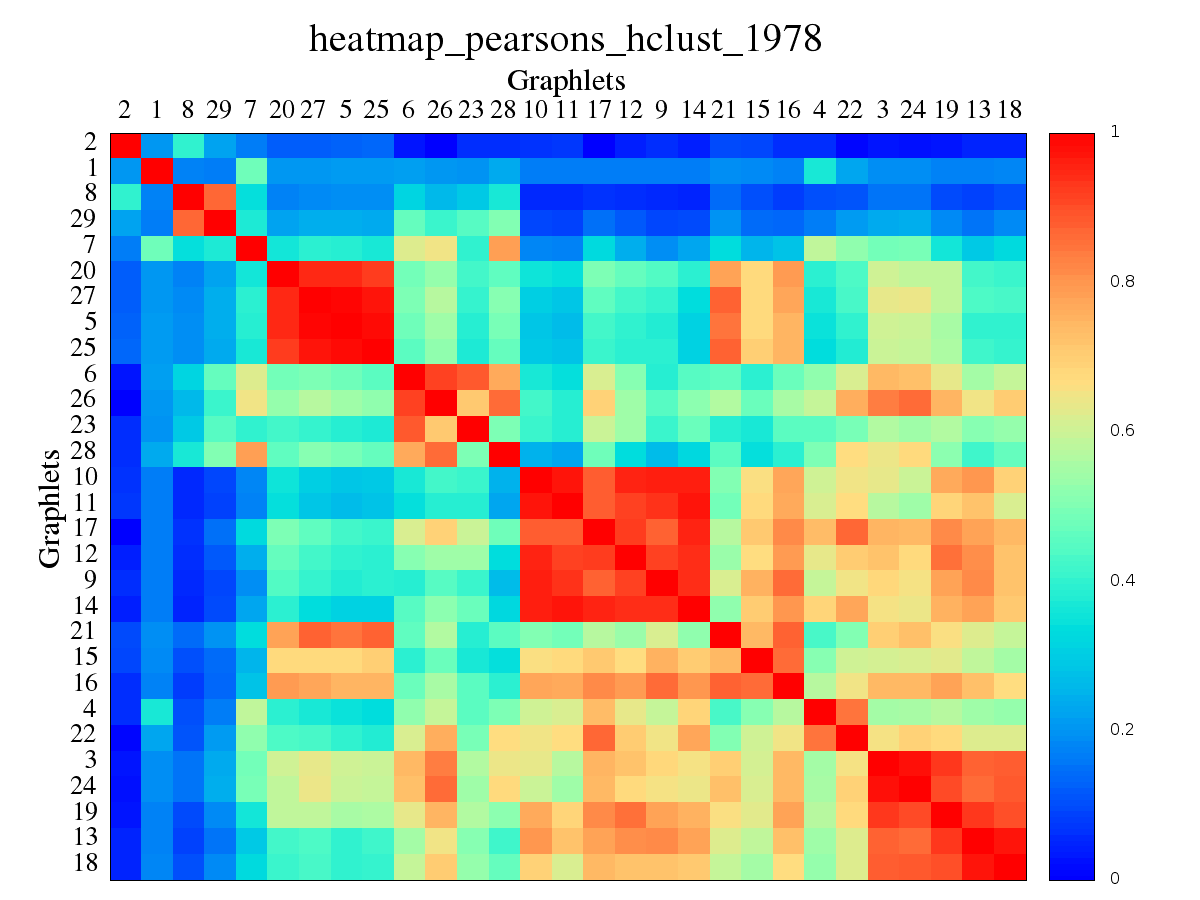
\includegraphics[width=70mm]{../code/final_results_norm1/all_trade_thresh/heatmap_pearsons_hclust_1978.png}}
  \subfloat{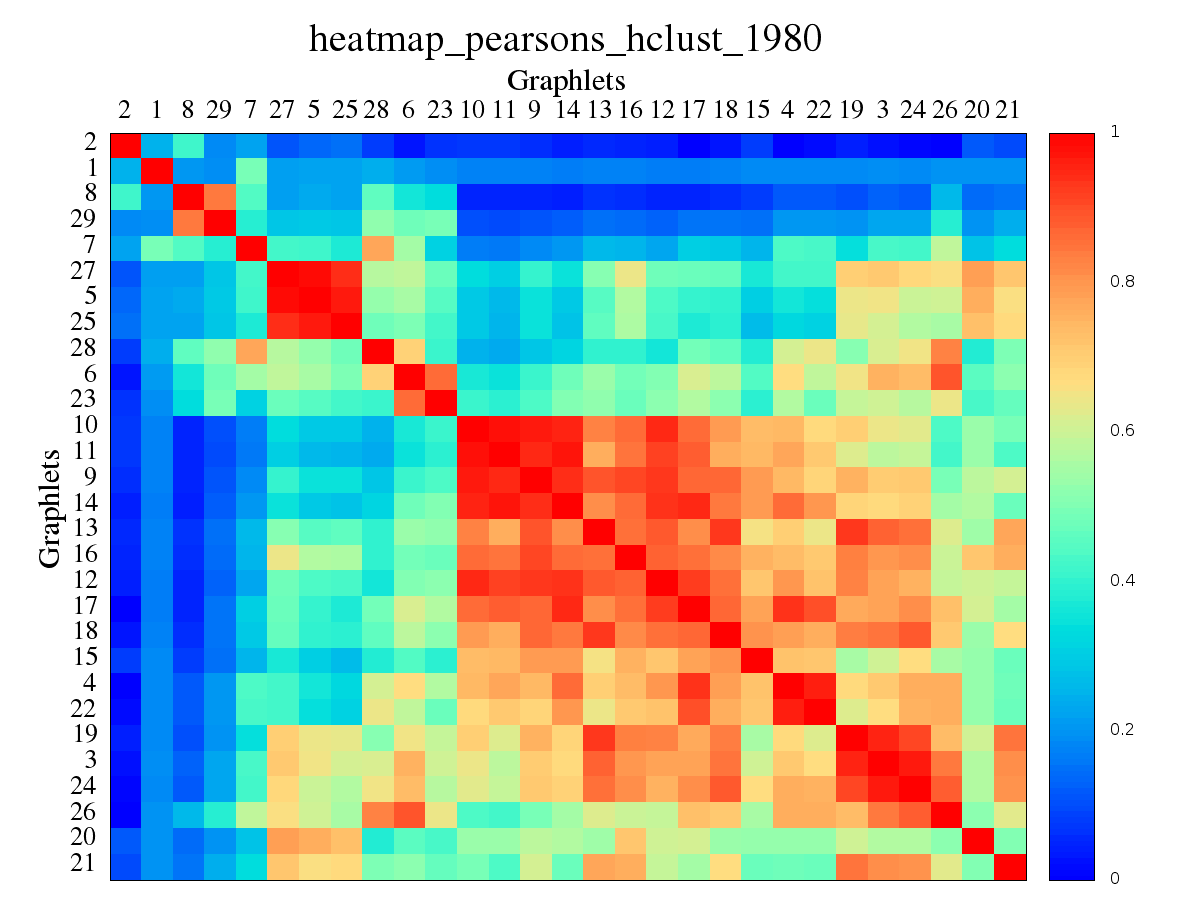
\includegraphics[width=70mm]{../code/final_results_norm1/all_trade_thresh/heatmap_pearsons_hclust_1980.png}}
  \\
  \subfloat{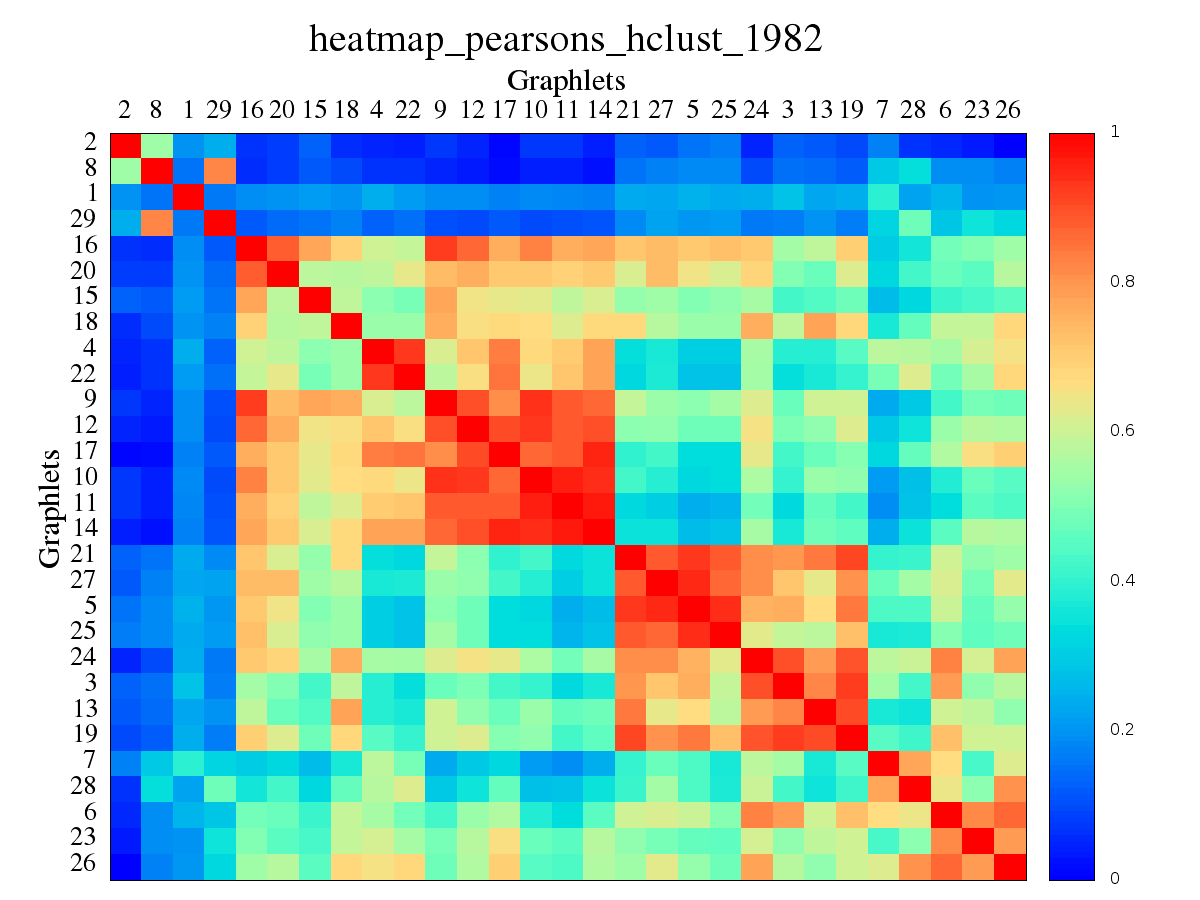
\includegraphics[width=70mm]{../code/final_results_norm1/all_trade_thresh/heatmap_pearsons_hclust_1982.png}}
  \subfloat{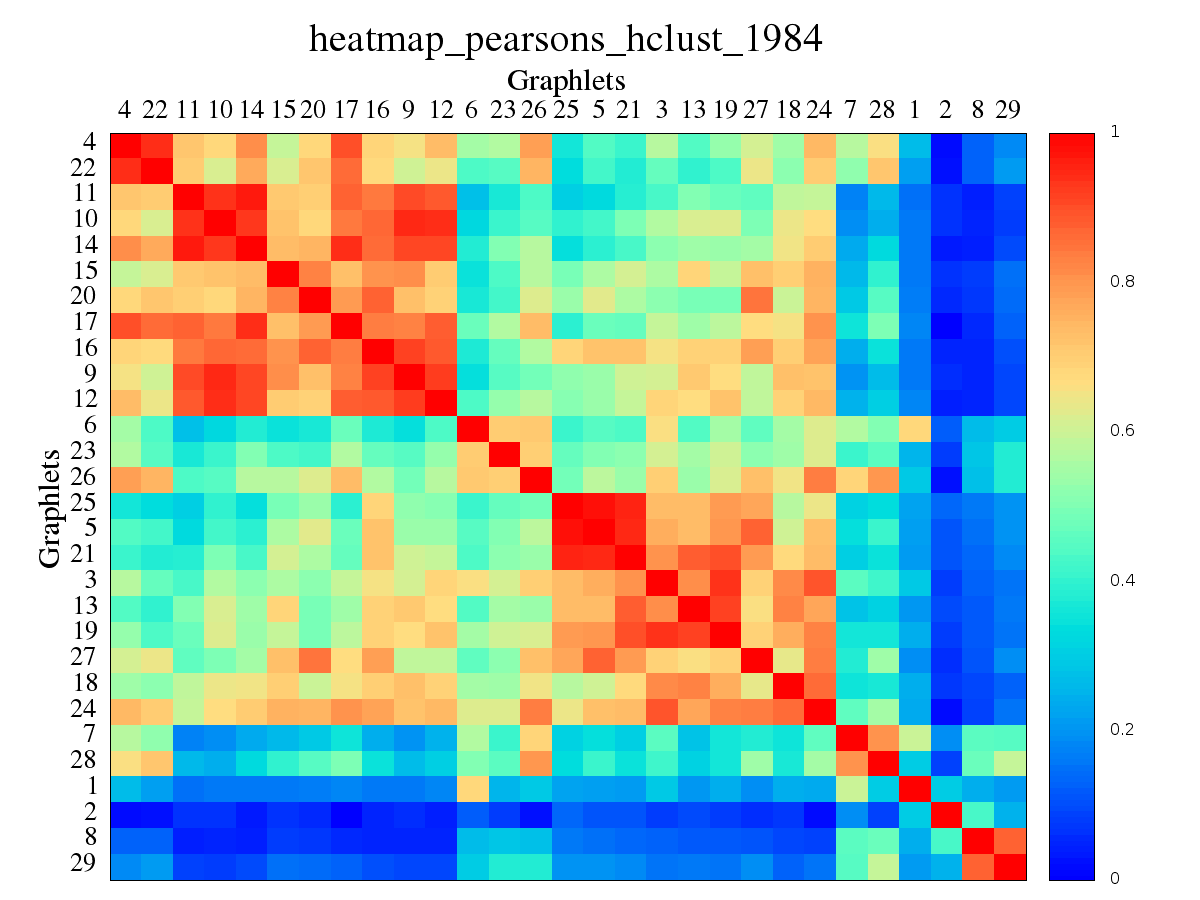
\includegraphics[width=70mm]{../code/final_results_norm1/all_trade_thresh/heatmap_pearsons_hclust_1984.png}}

\end{figure}


\subsection*{1986 to 1996}

\begin{figure}[H]
  \centering
  \label{fig:asafa}
  
  \subfloat{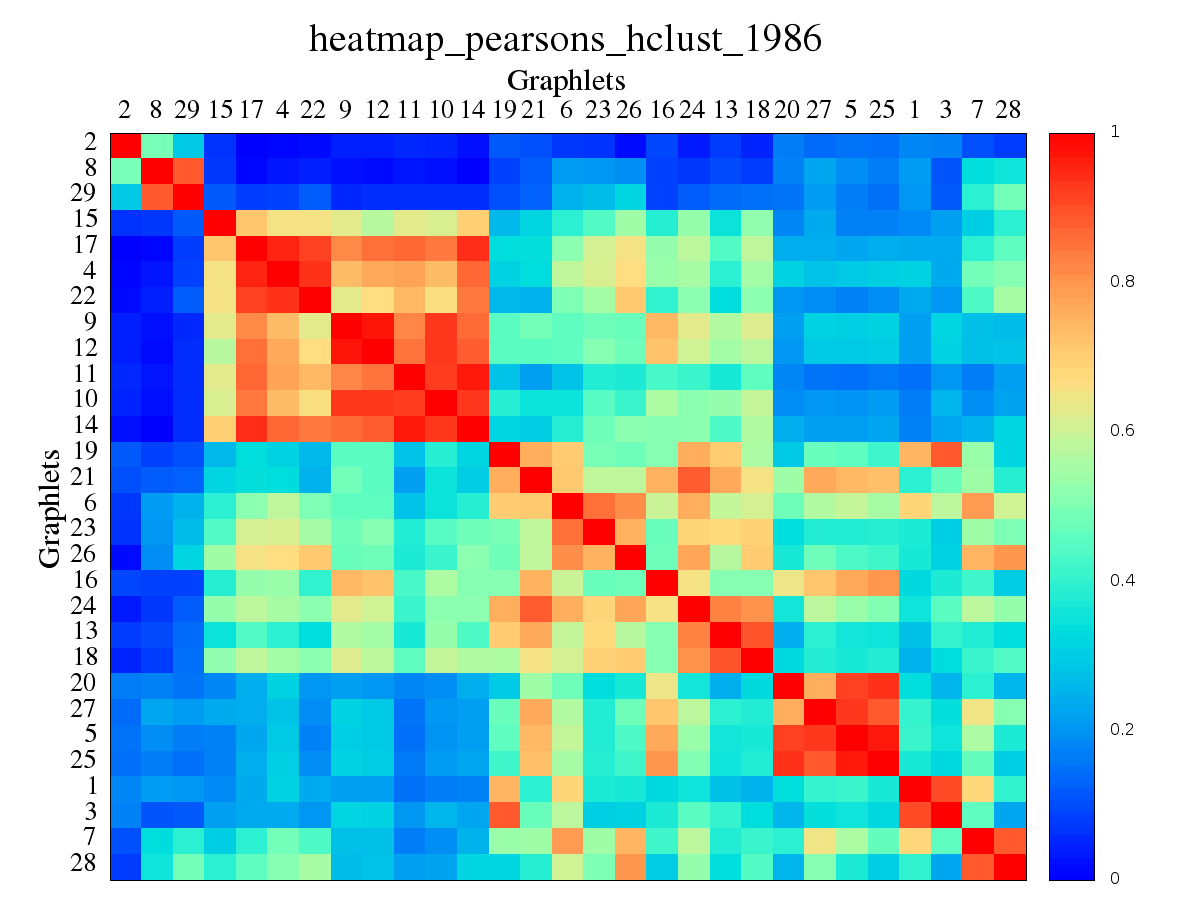
\includegraphics[width=70mm]{../code/final_results_norm1/all_trade_thresh/heatmap_pearsons_hclust_1986.png}}
  \subfloat{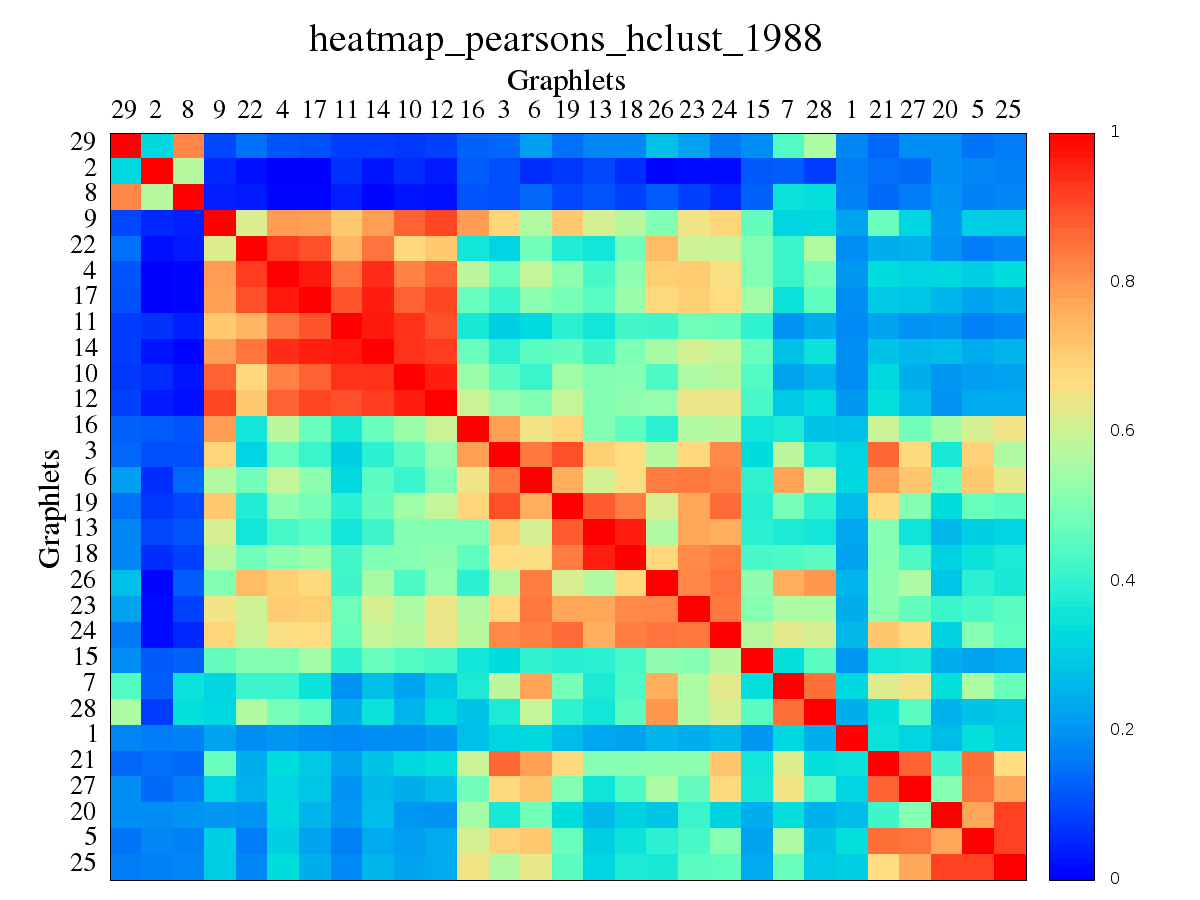
\includegraphics[width=70mm]{../code/final_results_norm1/all_trade_thresh/heatmap_pearsons_hclust_1988.png}}
  \\
  \subfloat{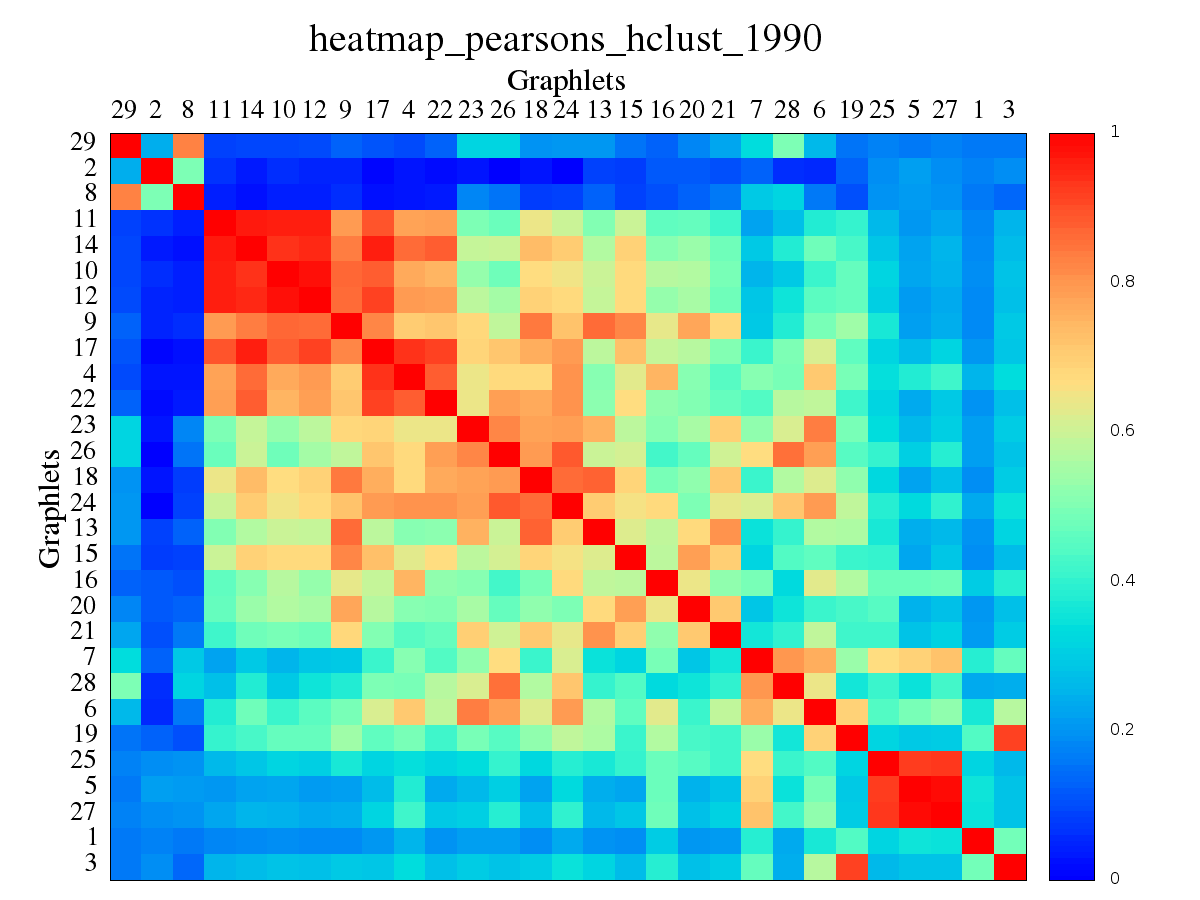
\includegraphics[width=70mm]{../code/final_results_norm1/all_trade_thresh/heatmap_pearsons_hclust_1990.png}}
  \subfloat{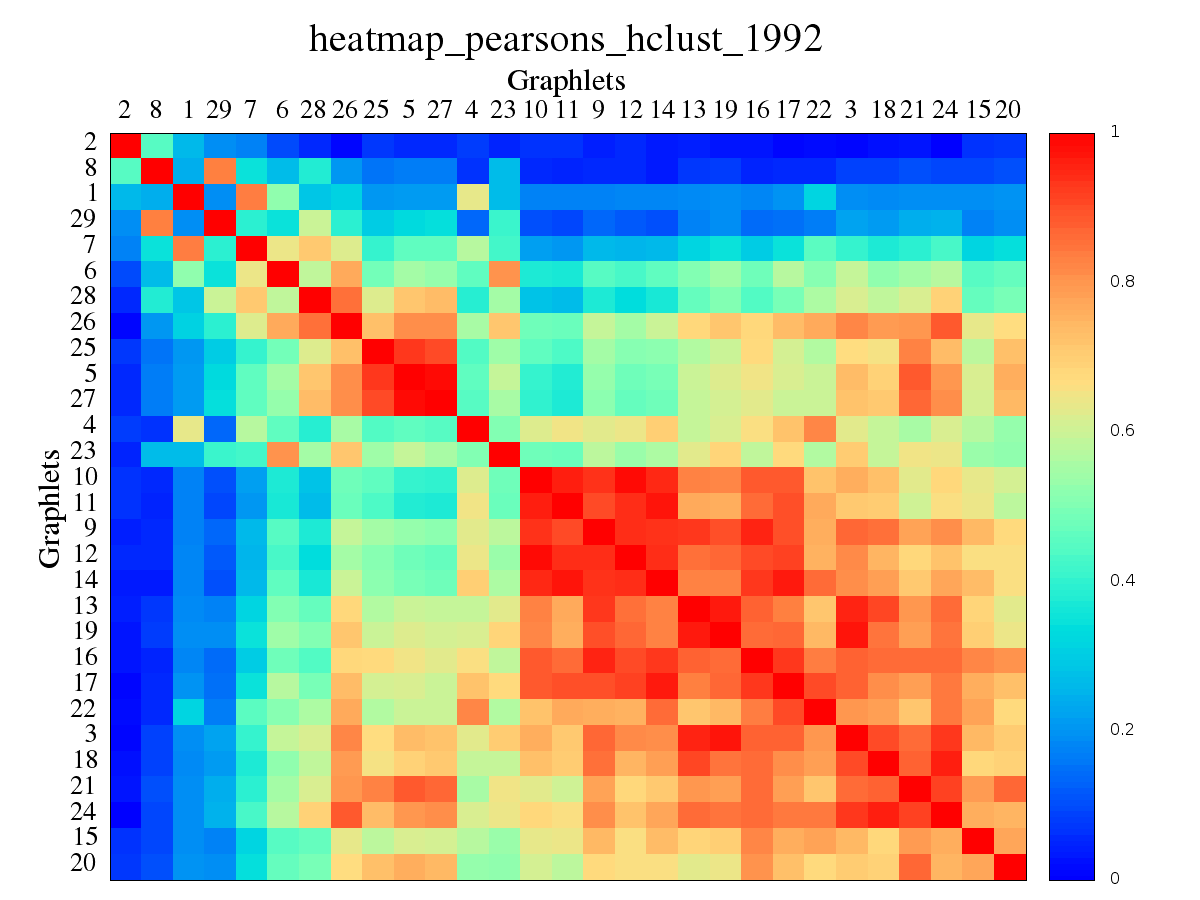
\includegraphics[width=70mm]{../code/final_results_norm1/all_trade_thresh/heatmap_pearsons_hclust_1992.png}}
  \\
  \subfloat{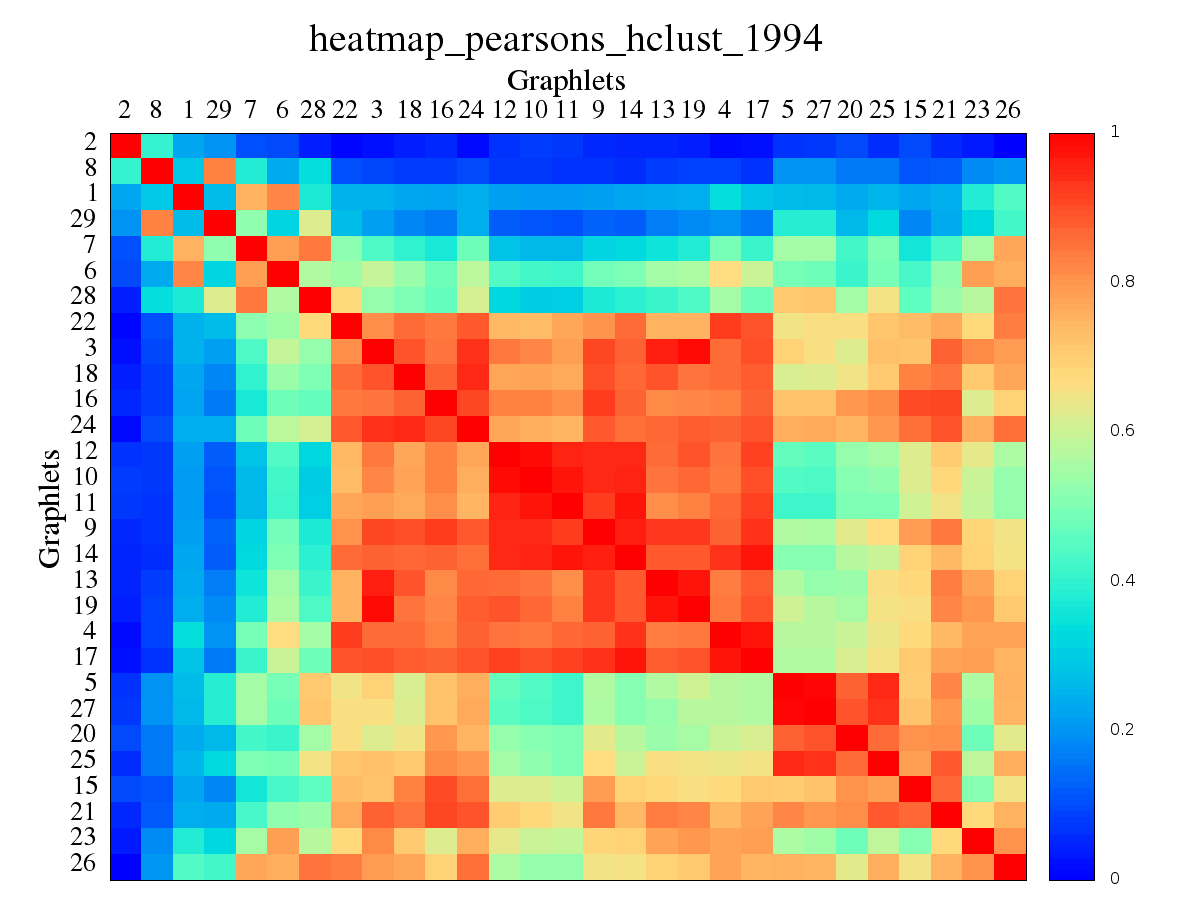
\includegraphics[width=70mm]{../code/final_results_norm1/all_trade_thresh/heatmap_pearsons_hclust_1994.png}}
  \subfloat{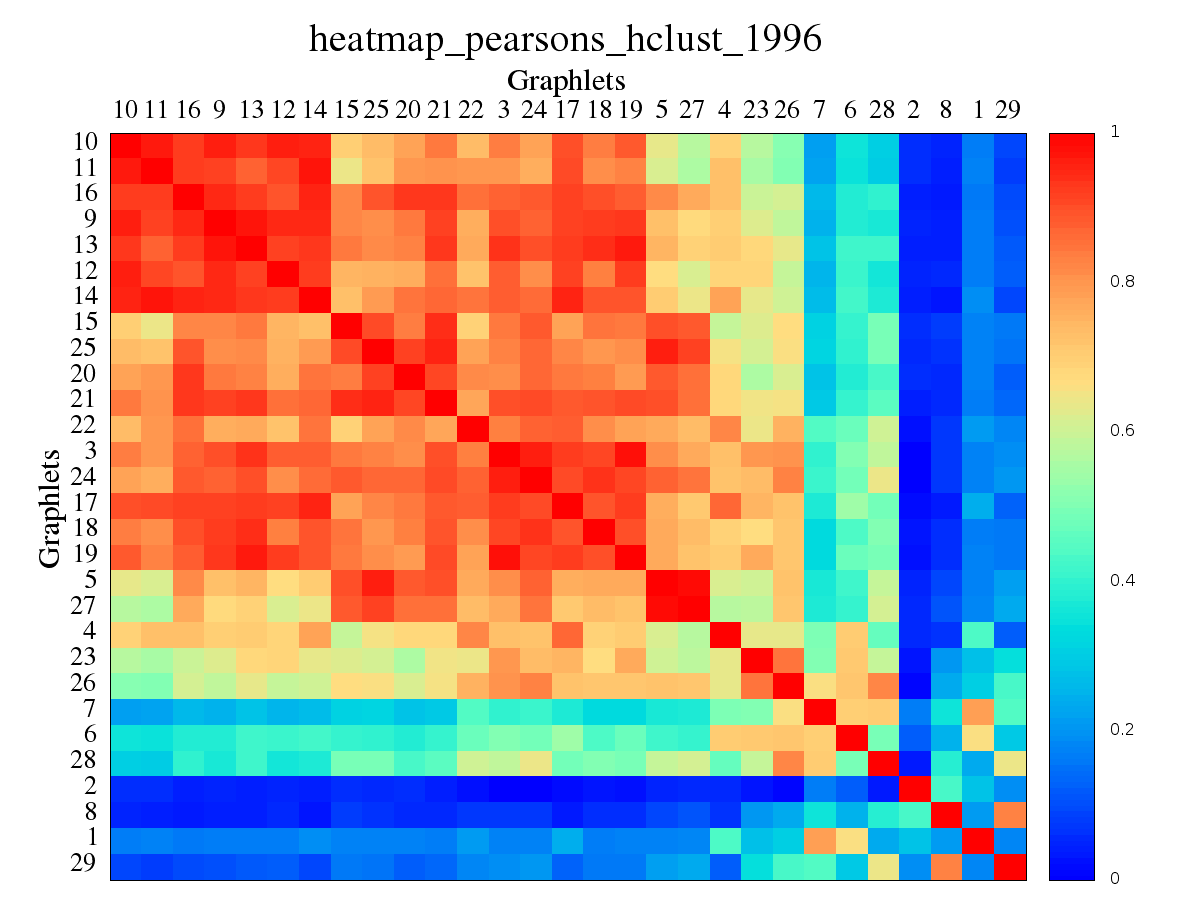
\includegraphics[width=70mm]{../code/final_results_norm1/all_trade_thresh/heatmap_pearsons_hclust_1996.png}}

\end{figure}



\appendix
% these do NOT count as part of the suggested page count
% This is probably a good place to explain the models in some detail for example



\subsection*{Canonical correlation analysis on Economic Integration}

I have tried to analayse whether the level of \emph{Economic Integration} of a country is positively correlated with dense graphlets and negatively correlated with sparse graphlets. This is something to be expected, since when a country is part of a strong trading bloc, then it's neighbours have a higher probability of doing heavy trade with one another. This is because there is incentive for the country to trade more with the partners from the same bloc. This would in turn result in denser graphlets in the neighbourhood of that country. 

I have therefore annotated each country with a number (1-6) that measures the degree of economic integration:
\begin{itemize}
 \item 0 - no economic integration 
 \item 1 - Multilateral Free Trade Area (AFTA, CEFTA, CISFTA, COMESA, GAFTA, GCC
 \item 2 - Customs union (CAN, CUBKR, EAC, EUCU, MERCOSUR, SACU)
 \item 3 - Common market (EEA, EFTA, CES) 
 \item 4 - Customs and Monetary Union (CEMAC/franc, UEMOA/franc) 
 \item 5 - Economic union (CSME, EU) 
 \item 6 - Economic and monetary union (CSME/EC dollar, EU euro)
\end{itemize}


\begin{tabular}{ c | l }
canonical correlation &  0.618823452163313\\
p-value (asymptotic Wilks): & 0.0128012383082338\\
\hline
"Integration" & 0.618823452346073\\
\hline
\textbf{"sig29"} & 0.287035191288073\\
\textbf{"sig8"} & 0.283489421651237\\
\textbf{"sig2"} & 0.278615840865378\\
"sig22" & 0.26819674644438\\
"sig28" & 0.268059123234175\\
"sig7" & 0.260207030053052\\
"sig26" & 0.260112720674704\\
"sig18" & 0.246614831141233\\
"sig1" & 0.238368565474503\\
"sig24" & 0.231333551025451\\
"sig6" & 0.229690387810875\\
"sig4" & 0.220206855982917\\
"sig27" & 0.220129084450554\\
"sig17" & 0.210208580507573\\
"sig14" & 0.206306944610344\\
"sig23" & 0.204204021795578\\
"sig5" & 0.201486106029494\\
"sig20" & 0.193906989388751\\
"sig25" & 0.191223668928417\\
"sig21" & 0.190762668949242\\
"sig16" & 0.190257968164896\\
"sig11" & 0.183299329835195\\
"sig3"& 0.177301380839247\\
"sig15"& 0.168139476991408\\
"sig13"& 0.16763975453569\\
"sig19"& 0.160509773821264\\
"sig9" &0.150872182634174\\
"sig12"& 0.148861465107402\\
"sig10"& 0.146375591601729\\
\end{tabular}\\



\subsection*{Change over years}

\begin{figure}[H]
  \centering
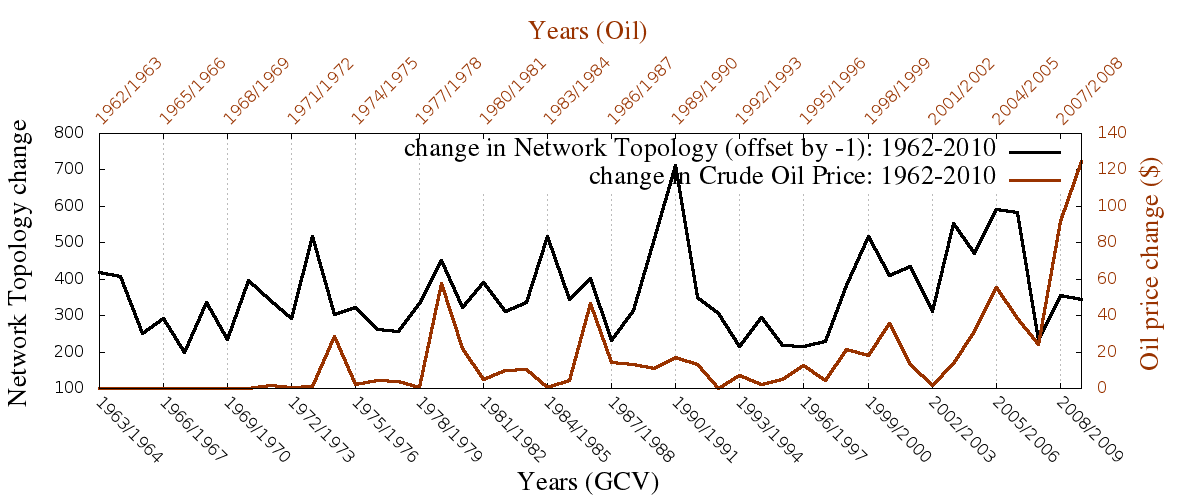
\includegraphics[scale=0.4]
{../code/final_results_norm1/all_trade_thresh/change_over_time.png}
\caption{}
\label{fig:hsa_meta}
\end{figure}

Important economic events that match the graph:
\begin{itemize}
 \item OPEC oil crisis 1973 (although the peak in our graph occurs 3 years earlier)
 \item 1990's revolutions in Eastern Europe that mark a starting point of 
 increasing trade between Western Europe and Eastern Europe. Transition to a capitalist-like economy happened thoughout the world.
\end{itemize}

1970s were marked by energy crises that (1973 and 1979) which might explain the two small peaks. 

The 1984 peak could be potentially explained by the early 1980 recession, which affected most of the developed world. Revival of neoliberalist economic policies occured in this time which led to reduced government intervention, lower taxes and deregulation. The peak in 1989 might be explained by the fall of communist/socialist governments in Russia, Eastern Europe and around the world accompanied by a fall in heavy industries and increased trade openness.

Our plot shows the early 90s as a period of relative stability in the Western world, which reflects the economic situation at that time. However, bigger changes are noticed in the late 90s, possibly started by the 1997 Asian financial crisis. 

By the 2000s, the changes could be potentially caused by the commodities boom (and especially rising oil prices) and rising inflation. 

\subsection*{Food and live animals - CCA results}


\begin{tabular}{ c | l }
canonical correlation &  0.931343399676811\\
p-value & 0.0\\
\hline
"POP" & 0.768789219153116\\
"LE" & 0.75589193067634\\
"KGxRGDPLxPOP" & 0.724041566642826\\
"RGDPLxPOP" & 0.712700750050226\\
"RGDPCHxPOP" & 0.712674980119381\\
"RGDPL2xPOP" & 0.712492101319333\\
"KCxRGDPLxPOP" & 0.699062250542676\\
"KIxRGDPLxPOP" & 0.692573818759865\\
"KCxRGDPL" & 0.379230434013614\\
"KGxRGDPL" & 0.280897452435245\\
"KC" & 0.221181934910442\\
"RGDPL" & 0.201678920057773\\
"RGDPCH" & 0.201204841445596\\
"RGDPL2" & 0.199863198064912\\
"KIxRGDPL" & 0.0431392035994932\\
"KG" & -0.0274551245914152\\
"XRAT" & -0.0580790619503796\\
"BCAperRGDPL" & -0.200304005013981\\
"BCA" & -0.226719786693096\\
"KI" & -0.242826899387707\\
"OPENK" & -0.331085303964667\\
\hline
"sig10" & 0.88692337144164\\
"sig12" & 0.83067416094356\\
"sig9" & 0.829092446025452\\
"sig14" & 0.813403862498435\\
"sig11" & 0.788793605804233\\
"sig16" & 0.769229375658728\\
"sig13" & 0.743377980660789\\
"sig17" & 0.742559765169964\\
"sig19" & 0.659965113520015\\
"sig18" & 0.551426156240859\\
"sig4" & 0.544092889184998\\
"sig24" & 0.493047720478224\\
"sig21" & 0.492123130860659\\
"sig22" & 0.465992488592433\\
"sig3" & 0.438525664876755\\
"sig20" & 0.331070823091142\\
"sig15" & 0.330193853619742\\
"sig23" & 0.312108214450326\\
"sig25" & 0.203540813559098\\
"sig26" & 0.120938760781583\\
"sig27" & 0.119339209986085\\
"sig5" & 0.0247087925928628\\
"sig6" & -0.0527788861234204\\
"sig28" & -0.153460808568266\\
"sig1" & -0.219580042055988\\
"sig7" & -0.300506776390814\\
"sig29" & -0.339373603003912\\
"sig2" & -0.421218901897477\\
"sig8" & -0.429682161840808\\
\end{tabular}\\


\subsection*{Minerals and fuels - CCA results}


\begin{tabular}{ c | l }
canonical correlation &  0.948736157470611\\
p-value & 0.0\\
\hline
"POP" & 0.876457874567787\\
"LE" & 0.863682777597727\\
"KGxRGDPLxPOP" & 0.860343204523055\\
"RGDPL2xPOP"& 0.846874458743335\\
"RGDPLxPOP"& 0.846008041944914\\
"RGDPCHxPOP"& 0.845910737818323\\
"KCxRGDPLxPOP"& 0.839909495518377\\
"KIxRGDPLxPOP"& 0.818662713048328\\
"KCxRGDPL"& 0.286222414674107\\
"KGxRGDPL"& 0.263523493822553\\
"RGDPL2"& 0.189581025897181\\
"RGDPCH"& 0.188547823752884\\
"RGDPL"& 0.188489993954331\\
"KIxRGDPL"& 0.129223611296276\\
"XRAT"& 0.0893558131038519\\
"KC"& 0.0358681762868585\\
"KI"& -0.0142215263251962\\
"KG"& -0.0269184534621442\\
"OPENK"& -0.151550855268402\\
"BCAperRGDPL"& -0.406585541496086\\
"BCA"& -0.43176995068358\\
\hline
"sig9"& 0.872148579806222\\
"sig10"& 0.868973766269167\\
"sig16"& 0.791817611528138\\
"sig13"& 0.776486977955135\\
"sig12"& 0.674079322848685\\
"sig19"& 0.589485447723753\\
"sig21"& 0.525353468439205\\
"sig17"& 0.488849900019008\\
"sig20"& 0.483156902006927\\
"sig14"& 0.470227100086494\\
"sig15"& 0.457636105722408\\
"sig23"& 0.38372712438183\\
"sig11"& 0.379413005944458\\
"sig18"& 0.347285452681086\\
"sig25"& 0.340549909317534\\
"sig24"& 0.294343038658771\\
"sig3"& 0.256411491615714\\
"sig22"& 0.251168790392317\\
"sig4"& 0.215861163396094\\
"sig26"& 0.210767880510244\\
"sig5"& 0.16342056884694\\
"sig6"& 0.140553091466648\\
"sig27"& 0.123420111132331\\
"sig28"& 0.0636859586652647\\
"sig29"& -0.0125965761044901\\
"sig7"& -0.0289952308406711\\
"sig8"& -0.102949228155779\\
"sig2"& -0.201272249268219\\
"sig1"& -0.215614091716047\\
\end{tabular}\\

\subsection*{Economic interpretation}

The conclusions we draw from the CCA analysis of comodity trade are similar to the ones from the total trade. More precisely, sparse graphlets such as \{9,10,11,12,13,16\} are correlated with good indicators, while denser graphlets such as cliques \{ 2,8 and 29 \} are assciated with poor countries. This implies that \textbf{rich countries have trading partners that include small, isolated countries which trade less with each other, while poor countries often only trade with the big economic groups such as G8,G20, OECD which perform a lot of trade with each other}.

\section*{Metabolic Networks}

\textbf{Enzyme} - calculated correlation matrices + CCA on 5 organisms - no results at all.\\
\textbf{Compound} - Heatmaps have some faint clusters + CCA only got some correlation with EC6, as before.\\ 

I would recommend not going any deeper into metabolic networks.\\


\subsection*{Hsa metabolic Network (Compound-based)}

\begin{figure}[H]
  \centering
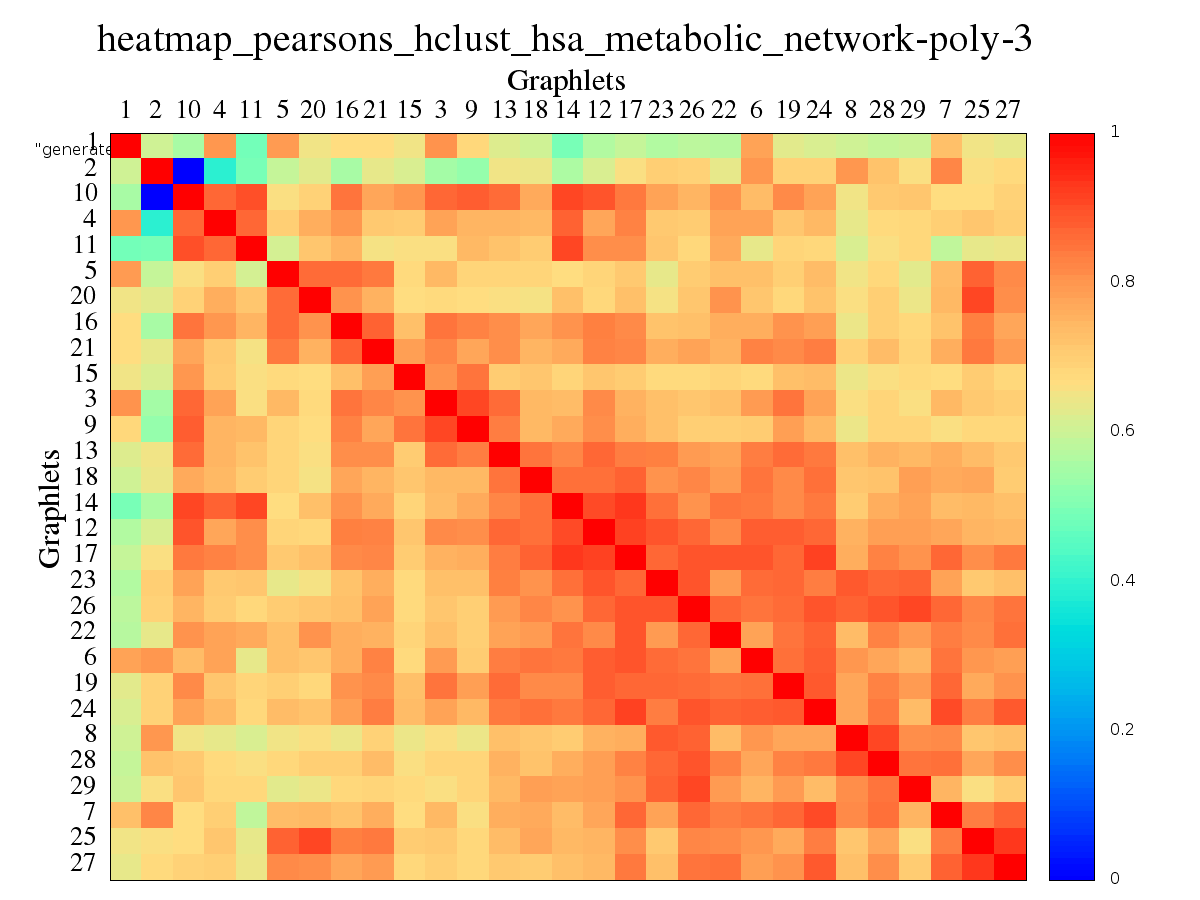
\includegraphics[scale=0.4]
{../code/final_results_norm1/hsa_metabolic_network/heatmap_pearsons_hclust_hsa_metabolic_network-poly-3.png}
\caption{}
\label{fig:hsa_meta}
\end{figure}

\subsection*{Enzyme-based metabolic networks}

I have analysed plotted heatmaps and ran Canonical Correlation analysis on other metabolic networks that belong to the following organisms: C. elegans, D.melanogaster, E.coli, M.musculus, S.cerevisiae. 

Heatmaps have no clusters and CCA yielded no correlation whatsoever (big p-value).

\section*{PPI networks}
\subsection*{Human PPI}

Heatmaps: clusters are faint
CCA analysis - graphlet separation is still noticeable, although to a much lesser extent. 

A few things might be said about these networks, but the results are definitely inferior to the trade networks.

\begin{figure}[H]
  \centering
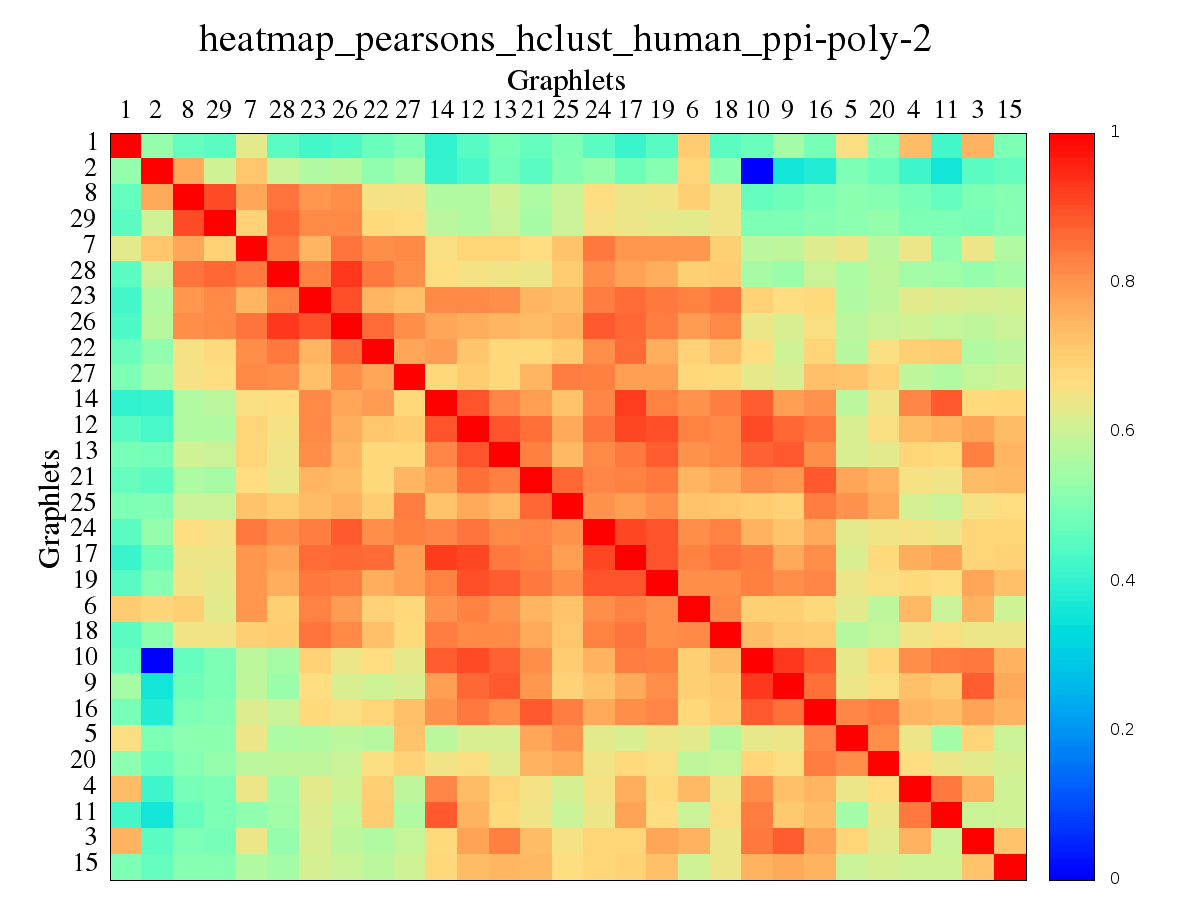
\includegraphics[scale=0.4]
{../code/final_results_norm1/human_ppi/heatmap_pearsons_hclust_human_ppi-poly-2.png}
\caption{}
\label{fig:human_ppi}
\end{figure}


\subsection*{The 18 experiments}

We performed CCA on 6 different human ppi networks with one annotation file and also on 6 yeast networks using 2 annotation files. The networks were as follows:

\begin{itemize}
 \item Human - one annotation file (14) -- 6 experiments in total
 \begin{enumerate}
    \item human HI 2012 preliminary
    \item human i2d full
    \item human i2d hc
    \item human ppi 56k
    \item biogrid human ppi noUBC full (removed the ubiquitous protein)
    \item biogrid human ppi hc
  \end{enumerate}
 \item Yeast - two annotation files: boone (14) and merin (13) -- 6x2 = 12 experiments in total
  \begin{enumerate}
    \item yeast apms collins
    \item yeast biogrid genetic
    \item yeast lc
    \item yeast y2h union yu ito uetz
    \item biogrid yeast ppi noYLL039C full (removed the ubiquitous protein)
    \item biogrid yeast ppi hc
  \end{enumerate}
\end{itemize}

 
\section*{Literature networks}

\subsection*{Anna Karenina - Knuth literature}

\begin{figure}[H]
  \centering
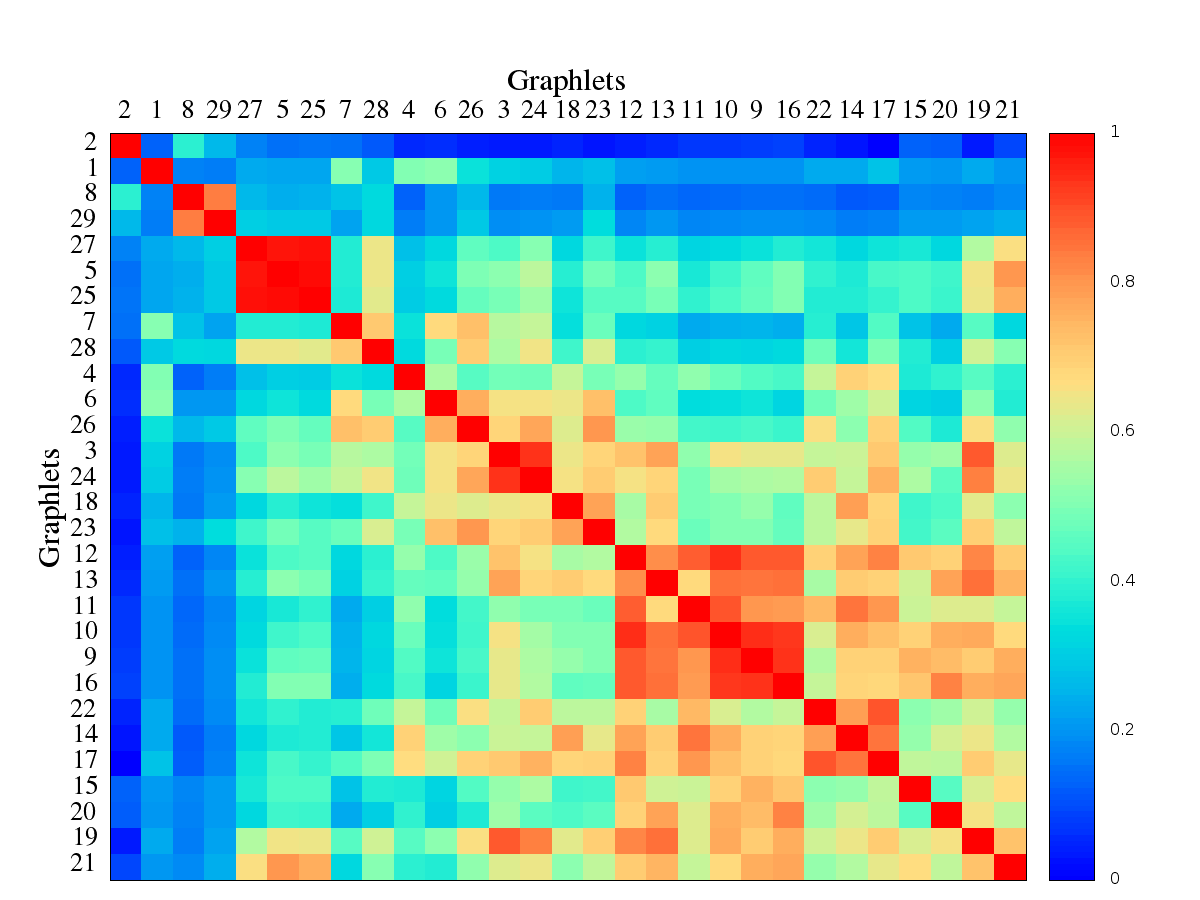
\includegraphics[scale=0.4]
{../code/final_results_norm1/knuth_literature/anna/heatmap_pearsons_hclust_anna.png}
\label{fig:anna-knuth}
\caption{Anna karenina - Hierarchically clustered, normalised with simple feature scaling}
\end{figure}



\subsection*{David Copperfield - Knuth literature}

\begin{figure}[H]
  \centering
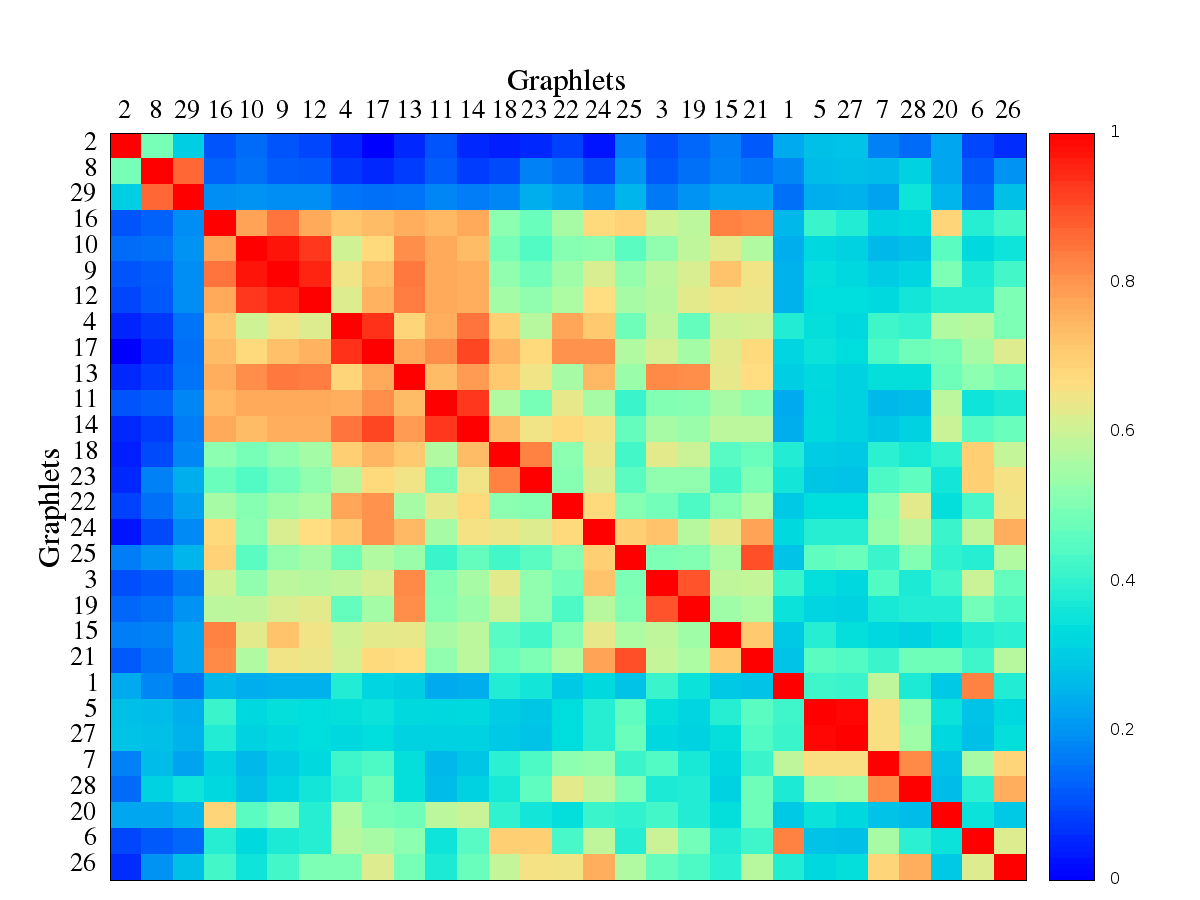
\includegraphics[scale=0.4]
{../code/final_results_norm1/knuth_literature/david/heatmap_pearsons_hclust_david.png}
\caption{David Copperfield - Hierarchically clustered, only normalised with simple feature scaling}
\label{fig:anna-knuth}
\end{figure}


Other literature networks for which I have calculated the heatmaps are:
\begin{itemize}
 \item Knuth Literature:
 \begin{itemize}
    \item Homer - Iliad or Odyssey
    \item Adventures of Huckleberry Finn
    \item Jean (??)
  \end{itemize}
 \item Mreze Literature:
 \begin{itemize}
    \item Anna Karenina
    \item David Copperfield
    \item Les Miserables
  \end{itemize}
  \item Processing under way
  \begin{itemize}
  \item Bible
    \item Old Testament
    \item New Testament
  \end{itemize}
  \end{itemize}


\end{document}
